\section{Livello 3: Network}
        \subsubsection{Scopi e servizi del livello Network}
            Estendere i servizi che il livello data link offre a macchine connesse, anche a macchine non hanno una connessione diretta.

            Compito fondamentale dello strato di rete è trasportare i pacchetti lungo tutto il percorso dal mittente al destinatario, attraversando tutti i nodi di transito dove sono possibili scelte alternative per le linee di uscita.

            La funzione di collegamento di una linea di ingresso con una linea di uscita opportunamente scelta, che viene svolta nei nodi, è detta \textbf{Commutazione (Switching)}.

            Il routing è quella parte del software dello strato Network che si preoccupa dell'instradamento dei pacchetti in transito.

            Se la rete è \textit{a datagramma} il routing viene determinato per ogni pacchetto, poiché il percorso migliore può cambiare nel tempo.

            Se la rete è \textit{a circuito virtuale} il routing viene determinato al momento dell'attivazione del circuito. Da quel momento in poi tutti i pacchetti seguono il percorso stabilito.

        \subsubsection{Commutazione di circuito}
            I nodi di transito sono i centralini di commutazione (manuali, meccanici o elettronici).
        
            L'algoritmo per la commutazione interviene all'apertura del canale fisico: nella fase di connessione vengono allocate le risorse necessarie.
        
            Il ritardo è minimo nel trasferimento dati, ma elevato in fase di apertura e chiusura della connessione.
        
            Le risorse allocate sono riservate anche se la connessione non è utilizzata, questo non avviene per le telefonate, ma può avvenire per il trasferimento dati.

        \subsubsection{Commutazione di pacchetto}
            La comunicazione viene frazionata in pacchetti, l'algoritmo di per la commutazione interviene sui pacchetti.
        
            Esistono diversi tipi di nodi transito a seconda della loro funzione (hub, bridge, router, gateway).
        
            Esistono due tipologie di commutazione di pacchetto:
            \begin{itemize}
                \item \textbf{A circuito virtuale}: l'algoritmo per la commutazione interviene solo all'inizio dell'apertura del Virtual Channel (VC).
                Ogni router viene marcato con l'etichetta del VC ed i pacchetti seguono il percorso individuato. Le implementazioni principali sono:
                \begin{itemize}
                    \item ATM : è la rete a pacchetto per la telefonia.
                    \item Tramite il protocollo MPLS.
                    \item IPv6.
                \end{itemize}
                \item \textbf{A datagramma}: i pacchetti sono instradati in modo indipendente in base all'indirizzo di destinazione.
                
                L'instradamento è determinato dai router attraversati in base a delle tebelle di routing, che ogni router costruisce dinamicamente tramite algoritmi di routing.
                
                I pacchetti della stessa connessione possono seguire percorsi diversi. Le implementazioni principali sono IPv4 e IPv6.
            \end{itemize}

    \subsection{Reti a circuito virtuale: MPLS}
        \textbf{MPLS (Multi-Protocol Label Switching)} consente di creare aree a commutazione di label.
    
        È uno strato che si pone sotto il livello di rete, aggiugendo un proprio Header di 4 byte tra l'header del livello rete (IP), e quello del livello data link (PPP o Ethernet). Viene considerato, infatti, un protocollo di livello 2.5.
    
        I campi principali sono la Label (20 bit), QoS, e TTL.

        \begin{center}
            \includegraphics[scale=0.4]{chapters/4/assets/schema_a.png}
        \end{center}
        
        Vantaggi del protocollo: QoS, Traffic Shaping (e-mail, web, etc.), VPN.

        \subsubsection{Routing MPLS}
            Richiede al proprio interno router specifici che supportano il protocollo: il router di frontiera (\textbf{edge router}), determina il percorso ed aggiungere l'header MPLS al pacchetto.
    
            Attraverso le etichette, il primo pacchetto definisce un tunnel nella rete MPLS: i pacchetti successivi della stessa connessione, seguono il percorso indicato dal primo pacchetto.

    \subsection{La famiglia dei protocolli TCP/IP}
        Non esiste una specifica per gli strati sotto a IP, in quanto relativi alla singola sottorete.
        
        IP svolge funzioni di rete ed instradamento dei pacchetti.
    
        TCP (o UDP) svolge funzioni di trasporto e di controllo della connessione end-to-end.
    
        \begin{center}
            \includegraphics[scale=0.45]{chapters/4/assets/schema_b.png}
        \end{center}

        \subsubsection{Standard di Internet}
            Non esistono veri e propri enti che svolgono la funzione di gestione, ma solo enti di coordinamento delle attivit`a di ricerca e di sviluppo che ora convergono nella \textbf{Internet Society}. Dalla IS dipende l'Internet Advisory Board (IAB) e si compone di due sottogruppi:
            \begin{itemize}
                \item Internet Research Task Force (IRTF): coordina le attività di ricerca.
                \item Internet Engineering Task Force (IETF): coordina le attività di ingegnerizzazione ed implementazione.
            \end{itemize}

            \textbf{ICANN} è l'ente no-profit che assegna gli indirizzi IP e l'identificatore di protocollo e gestisce il DNS di primo livello (Top-Level Domain).

            Funzione svolta operativamente da \textbf{IANA} che è una sua emanazione.

            Data la complessità della gestione, sono state individuate 5 organizzazioni denominate: \textbf{RIR (Regional Internet Registries)} che in cooperazione con IANA hanno il compito di gestire le allocazioni a livello continentale.

        \subsubsection{Principi Architetturali di Internet}
            Descritti in ordine di importanza:
            \begin{enumerate}
                \item Assicurarsi che funzioni
                \item Mantenerlo semplice (nel dubbio, la soluzione più semplice)
                \item Fare scelte chiare (se si può fare in diversi modi sceglierne uno) 
                \item Sfruttare la modularità
                \item Aspettarsi l'eterogeneità
                \item Evitare opzioni e parametri statici
                \item Mirare ad un buon progetto (non necessariamente perfetto)
                \item Essere rigorosi nell'invio e tolleranti nella ricezione
                \item Pensare alla scalabilità (IPv4 e IPv6..)
                \item Considerare le prestazioni e i costi
            \end{enumerate}
    
    \subsection{IP: lo stato Network di Internet}
        Interconnette più reti di livello data link (LAN o connessioni punto-punto). Fornisce uno servizio per il trasporto di datagrammi (pacchetti) tra mittente e destinatari indipendentemente dalle loro reti di appartenenza. La versione del protocollo IP attualmente in uso, è IPv4.
    
        Operazioni:
        \begin{itemize}
            \item Lo stato di trasporto prende il flusso di dati e li divide in \textbf{datagrammi} che passa allo stato IP. La dimensione massima è di 64 KB, ma generalmente vengono scelti datagrammi non superiori a 1500 byte (per compatibilità con Ethernet).
            \item Il datagramma di trasporto (detto \textbf{segmento}) viene incorporato nella trama IP e trasferito da un router all'altro fino a destinazione.
            \item Il datagramma può subire una frammentazione nel caso di passaggio attraverso un livello data link con dimensione massima (MTU) inferiore. I frammenti vengono riassemblati a destinazione.
            \item Il datagramma (eventualmente riassemblato) viene estratto dalla trama IP e passato al livello di trasporto, che ricostruisce il flusso.
            \item QoS: La consegna è di tipo Best Effort.
        \end{itemize}

        \subsubsection{La trama IP}
            Il datagramma IP è costituito dall'intestazione (header) IP, seguita dal segmento di livello trasporto.

            \begin{center}
                \includegraphics[scale=0.33]{chapters/4/assets/schema_c.png}
            \end{center}

            L'header ha una parte fissa ed una parte opzionale variabile, trasmessa in ordine big endian.

            \begin{center}
                \includegraphics[scale=0.34]{chapters/4/assets/schema_d.png}
            \end{center}

            Significato dei campi del pacchetto IP:
            \begin{itemize}
                \item \textbf{Version} (4 bit): i primi 4 bit di ogni pacchetto IP contengono il numero di versione.
                \item \textbf{HLEN} (4 bit): dimensione dell'header espressa in parole di 4 byte.
                \item \textbf{Type Of Service} (4 bit): inizialmente per controllo della rete, successi-
                vamente codifica classi di servizio, poco utilizzato.
                \item \textbf{Total Lenght} (16 bit): numero di byte totali (header più dati) (mssimo 64 KB).
                \item \textbf{Identification} (16 bit): tutti i frammenti del datagramma hanno lo stesso valore.
                \item \textbf{DF} (1 bit): Don't Fragment: ordina ai router di non frammentare.
                \item \textbf{MF} (1 bit): More Fragment: impostato ad 1 per tutti i frammenti tranne
                l'ultimo.
                \item \textbf{Fragment Offset} (13 bit): indica la posizione del frammento nel datagramma corrente, espressa in blocchi di 8 byte.
                \item \textbf{TTL} (8 bit): numero massimo di salti; si decrementa ad ogni passaggio; quando arriva a 0 il pacchetto viene eliminato.
                \item \textbf{Protocol} (8 bit): protocollo di livello superiore (ICMP = 1, TCP = 6, UDP = 17, etc.).
                \item \textbf{Header Checksum} (16 bit): checksum dell'header, viene ricalcolato da ogni router, perché il TTL cambia ad ogni salto. Aiuta a rilevare errori generati da locazioni di memoria diffettose nel router, somma tutte le sequenze di 16 bit, con l'artimetica in complemento ad 1, e poi prende il complemento ad 1 del risultato.
                \item \textbf{Source e Destination Address} (32 e 32 bit): indirizzi di destinazione e sorgente.
                \item \textbf{Options}: pensato per poter aggiugnere estensioni non previste.
                \item \textbf{Padding}: bit aggiuntivi per rendere il campo Options multiplo di 32 bit.
            \end{itemize}

        \subsubsection{Indirizzi IP}
            Sono indirizzi a 32 bit con notazione dotted decimal: 4 decimali separati da un punto (.).
        
            Il numero massimo degli indirizzi è 232.
        
            Per motivi di routing, la sequenza è suddivisa in due parti:
            \begin{itemize}
                \item \textbf{NETid}: indentifica una rete di livello 2.
                \item \textbf{HOSTid}: distingue gli host della stessa rete.
            \end{itemize}

        \subsubsection{Classi IP}
            \begin{center}
                \includegraphics[scale=0.32]{chapters/4/assets/schema_e.png}
            \end{center}

            \begin{center}
                \includegraphics[scale=0.34]{chapters/4/assets/schema_f.png}
            \end{center}

        \subsubsection{Indirizzi IP speciali}
            \begin{center}
                \includegraphics[scale=0.36]{chapters/4/assets/schema_g.png}
            \end{center}

            Se la parte Host è di $N$ bit, il numero di indirizzi effettivamente assegnabili agli host è di $2N - 2$, poiché il primo indirizzo (tutti 0 nella parte host) indentifica la rete, mentre l'ultimo indirizzo (tutti 1 nella parte host), è l’indirizzo di broadcast.

        \subsubsection{Indirizzi IP per uso privato}     
            Le seguenti reti sono riservate da ICANN per uso privato (Intranet) e gli indirizzi non possono essere annunciati dai router.

            \begin{table}[h]
                \centering
                \begin{tabular}{|l|l|l|l|}
                \hline
                \rowcolor[HTML]{000000} 
                \multicolumn{1}{|c|}{\cellcolor[HTML]{000000}{\color[HTML]{EFEFEF} \textbf{Classi}}} & \multicolumn{1}{c|}{\cellcolor[HTML]{000000}{\color[HTML]{EFEFEF} \textbf{Inizio}}} & \multicolumn{1}{c|}{\cellcolor[HTML]{000000}{\color[HTML]{EFEFEF} \textbf{Fine}}} & \multicolumn{1}{c|}{\cellcolor[HTML]{000000}{\color[HTML]{EFEFEF} \textbf{Indirizzi}}} \\ \hline
                1 classe A & \verb:10.x.x.x: &  & 16M \\ \hline
                16 classi B & \verb:172.16.x.x: & \verb:172.31.x.x: & 1M \\ \hline
                255 classi C & \verb:192.168.0.x: & \verb:192.168.255.x: & 64M \\ \hline
                \end{tabular}
            \end{table}

            La rete \verb:169.254.0.0/16: è utilizzata dal servizio \textbf{Zeroconf} per assegnare un indirizzo IP agli host di una LAN senza dipendere da una infrastruttura, ovvero quando non è possibile ottenere un indirizzo dinamico da un server DHCP.

        \subsubsection{IP Subnetting}
            Consente di creare un ulteriore livello gerarchico per gli indirizzi IP: \textbf{NET-SUBNET-HOST}.
        
            Il \textbf{Netmask} è un parametro di 32 bit che stabilisce la suddivisione:
            \begin{itemize}
                \item Bit a 1 in corrispondenza del campo NET o SUBNET.
                \item Bit a 0 in corrispondenza del campo HOST.
            \end{itemize} 
        
        \subsubsection{Classless Inter-Domain Routing (CIDR)}
            Il numero di indirizzi IP è insufficiente; molte reti di classe B usano meno di 50 indirizzi.
        
            \textbf{CIDR} è una soluzione in attesa di IPv6: assegna gli indirizzi IPv4 rimanenti, in blocchi di dimensione variabile nella forma \textbf{netAddress/NetMaskBit}: il routing è più complicato perché si hanno tabelle più lunghe.
        
            Il supernetting consente di accorpare più reti contigue come fosse un'unica rete, ottimizzando i tempi di routing: in caso di sovrapposizioni tra due reti, vince quella che ha la netmask più lunga.

    \subsection{Instradamento dei datagrammi}
        La rete di appartenenza di un host è fondamentale per determinare la modalità di consegna, che può essere diretta o indiretta.
    
        La scelta del tipo di consegna avviene consultando la tabella di routing locale:
        \begin{itemize}
            \item Consegna diretta: host sorgente e destinatario condivido la stessa rete.
            \begin{itemize}
                \item trova l'indirizzo fisico del destinatario (con ARP), il quale viene associato all'indirizzo IP del destinatario.
                \item inoltra il pacchetto al livello link indirizzando il destinatario.
                \begin{table}[h]
                    \centering
                    \begin{tabular}{|c|l|l|l|l|}
                    \hline
                    \rowcolor[HTML]{000000} 
                    {\color[HTML]{EFEFEF} \textbf{N}} & \multicolumn{1}{c|}{\cellcolor[HTML]{000000}{\color[HTML]{EFEFEF} \textbf{Type}}} & \multicolumn{1}{c|}{\cellcolor[HTML]{000000}{\color[HTML]{EFEFEF} \textbf{To}}} & \multicolumn{1}{c|}{\cellcolor[HTML]{000000}{\color[HTML]{EFEFEF} \textbf{From}}} & \multicolumn{1}{c|}{\cellcolor[HTML]{000000}{\color[HTML]{EFEFEF} \textbf{Message}}} \\ \hline
                    1 & ARP Request & Broadcast & MACmitt & Who has IPdest? \\ \hline
                    2 & ARP Reply & MACmitt & MACdest & Me! \\ \hline
                    3 & Send IP & MACdest & MACmitt & xxxxxx \\ \hline
                    \end{tabular}
                \end{table}
            \end{itemize}

            \item Consegna indiretta: sorgente e destinatario appartengono a reti IP diverse.
            \begin{itemize}
                \item viene individuato il router da contattare, consultando la propria tabella di routing.
                \item trova l'indirizzo fisico del destinatario (con ARP), il quale viene associato all'indirizzo IP del destinatario.
                \item inoltra il pacchetto al livello link indirizzando il destinatario.
                \begin{table}[h]
                    \centering
                    \begin{tabular}{|c|l|l|l|l|}
                    \hline
                    \rowcolor[HTML]{000000} 
                    {\color[HTML]{EFEFEF} \textbf{N}} & \multicolumn{1}{c|}{\cellcolor[HTML]{000000}{\color[HTML]{EFEFEF} \textbf{Type}}} & \multicolumn{1}{c|}{\cellcolor[HTML]{000000}{\color[HTML]{EFEFEF} \textbf{To}}} & \multicolumn{1}{c|}{\cellcolor[HTML]{000000}{\color[HTML]{EFEFEF} \textbf{From}}} & \multicolumn{1}{c|}{\cellcolor[HTML]{000000}{\color[HTML]{EFEFEF} \textbf{Message}}} \\ \hline
                    1 & ARP Request & Broadcast & MACmitt & Who has IPdest? \\ \hline
                    2 & ARP Reply & MACmitt & MACrouter & \verb:dest:! \\ \hline
                    3 & Send IP & MACrouter & MACmitt & Send toIP: \verb:dest: \\ \hline
                    \end{tabular}
                \end{table}
            \end{itemize}
        \end{itemize}

        \subsubsection{Tabella di routing}
            È una tabella contenente le destinazioni, ed i percorsi per raggiungere tali destinazioni.
        
            Comando \verb:route: per Linux.
        
            Generalmente le reti locali hanno al proprio interno un router di riferimento (\textbf{Default Router}) a cui vengono consegnate tutte le destinazioni non note.
        
            La ricerca all'interno della tabella di routing avviene utilizzando l'IP di destinazione, e la rete di destinazione e \textit{netmask} di ciascuna riga della tabella.
        
            Se il risultato coincide con la rete presa in esame, la riga è quella giusta. Una volta trovato il risultato il lookup si ferma ed il datagramma viene instradata. Se nessuna riga corrisponde alla ricerca \verb:IpDest AND Mask:, si utilizza il router di default.
        
    \subsection{NAT}
        \textbf{NAT} è una tecnica dispositivo che consente agli host di una LAN (con indirizzi privati) di comunicare in Internet utilizzando un solo indirizzo pubblico.
    
        La linea verso Internet possiede un indirizzo IP pubblico e viene visto dagli host della LAN come Default Router.
    
        Le operazioni del NAT sono distinte in base alla direzione: \textbf{SNAT (Source-NAT)} è la funzionalità che consente di manipolare l'indirizzo sorgente ed è tipicamente utilizzato per consentire agli host di una LAN privata di uscire in internet.
    
        Quando un Host della LAN si rivolge al NAT per uscire in Internet il NAT trasforma l'indirizzo del mittente IP nell'indirizzo IP pubblico del NAT, quindi contatta il destinatario.
    
        \textbf{DNAT (Destination-NAT)} è utilizzata per manipolare l'indirizzo di destinazione. Viene usata tipicamente per dirottare verso un host interno le richieste provenienti da Internet.

        \subsubsection{Le tabelle del NAT}
            Le entry della tabella possono essere statiche o dinamiche:
            \begin{itemize}
                \item NAT dinamico: quando un client della LAN si rivolge al NAT per contattare un server esterno, il NAT genera una entry dinamica associando IP/porta del client con la IP/porta del server quindi applica SNAT. L'entry viene utilizzata per il DNAT sulla risposta del server.
                
                \begin{center}
                    \includegraphics[scale=0.35]{chapters/4/assets/schema_h.png}
                \end{center}

                \item NAT statico: Se vogliamo avere un server interno che deve essere contattato da un client esterno dobbiamo istruire il NAT mediante una entry statica che associa una porta del NAT con IP/porta del server interno. Quando un client esterno contatta il NAT sulla porta viene consultata la entry statica e applicato DNAT. Viene inoltre creata una entry dinamica che verrà utilizzata per applicare SNAT sulla risposta.
                
                \begin{center}
                    \includegraphics[scale=0.35]{chapters/4/assets/schema_i.png}
                \end{center}
            \end{itemize}

        \subsubsection{Problemi dell'architettura NAT}
            Viene violata l'univocità degli indirizzi: migliaia di host utilizzano gli stessi indirizzi privati.
        
            IP non è più connection-less, IP non è più stratificato: il Layer IP non dovrebbe entrare nei layer superiori.
        
            Un guasto al NAT, pregiudica tutte le connessioni che lo attraversano.
        
    \subsection{Protocollo ARP}
        Il protocollo \textbf{ARP (Address Resolution Protocol)}, ha il compito di determinare l'indirizzo fisico di un nodo IP.
    
        Quando un nodo mittente deve contattare un destinatario in Direct Delivery di cui ne conosce solo l'indirizzo IP, utilizza questo protocollo.
    
        Il funzionamento del protocollo è il seguente:
        \begin{itemize}
            \item Il nodo sorgente invia un pacchetto (\textbf{ARP Request}) con destinazione broadcast sulla LAN, contenente l'indirizzo IP del destinatario.
            \item I terminali con indirizzo IP diverso ignoreranno il pacchetto, mentre il nodo in oggetto rispondera (\textbf{ARP Reply}) con un Unicast, inviando il proprio indirizzo fisico.
            \item Ogni host mantiene una tabella (\textbf{ARP Cache}) con le corrispondenze ottenenute (comando \verb:arp -a:). Ogni entry ha un tempo di vita di 20 minuti.
        \end{itemize}

        Il frame ARP contiene un campo codice: 1 = ARPrequest, 2 = ARPreply, l'indirizzo IP e l'indirizzo fisico di partenza e destinazione.

    \subsection{Protocollo RARP}
        Il protocollo \textbf{RARP (Reverse ARP)} risolve il problema della conoscenza dell'indirizzo IP da parte di alcuni nodi della rete.
    
        Il client invia in broadcast il proprio indirizzo MAC, un server RARP con una tabella MAC-IP, risponderà con l'informazione richiesta.
    
        RARP presenta alcuni svantaggi: la richiestra Broadcast non passa i router, le associazioni MAC-IP sono statiche, non sono previste altre informazioni. \textit{DHCP} ha reso obsoleto \textit{RARP}.

    \subsection{Protocollo DHCP}
        Il protocollo \textbf{DHCP (Dynamic Host Configuration Protocol)} risolve lo stesso problema di RARP, aggiungendo nuovi servizi:
        \begin{itemize}
            \item il server DHCP può fornire informazioni al client: indirizzo IP, NetMask, Default Router, DNS Server, etc.
            \item l'indirizzo IP fornito può essere statico o dinamico.
            \item il server può riesiedere in una LAN diversa dalla LAN del client.
        \end{itemize}

        È un protocollo applicativo: utilizza la porta 67/UDP per il server, e la 68/UDP per il client.

        \subsubsection{Funzionamento DHCP}
            Il funzionamento è il seguente:
            \begin{itemize}
                \item Il client DHCP invia un pacchetto \textbf{DHCP Discover} in modalità broadcast.
                \begin{equation*}
                    \verb-0.0.0.0:68- ~ \rightarrow ~\verb-255.255.255.255:67-
                \end{equation*}
                \item Il server risponde con un pacchetto \textbf{DHCP Offer} che contiene l'indirizzo richiesto più eventuali informazioni.
                \begin{equation*}
                    \verb-Ipserver:67- ~ \rightarrow ~ \verb-Ipclient:68-
                \end{equation*}
            \end{itemize}

        \subsubsection{Funzionamento del DHCP: rinnovo}
            Il server gestisce una tabella in cui gli indirizzi IP possono essere associati staticamente ad indirizzi MAC oppure possono essere "affittati" dinamicamente al momento della richiesta, questo ha un termine: il client deve chiederne un eventuale rinnovo, altrimenti l'indirizzo viene ritirato ed assegnato ad un altro client.
        
            Le operazioni DHCP Request e DHCP Ack vengono ripetute per prolungare l'assegnazione dell'indirizzo.
        
            Per forzare il rinnovo su linux: \verb:dhclient -r && dhclient:
    
    \subsection{Protocollo ICMP}
        Il protocollo ICMP (Internet Control Message Protocol), permette lo scambio di messaggi di errore o di controllo che consentono agli host o ai router di accorgersi di eventuali malfunzionamenti della rete.

        Spedisce i messaggi di notifica dell'errore sempre al mittente del datagramma per il quale si è verificato l'errore.

        \subsubsection{Formato dei frame ICMP}
            Il formato del frame è costituito da una intestazione e da un'area dati. La prima è composta da tre campi:
            \begin{itemize}
                \item \textbf{TYPE}: è un numero di 8 bit che indentifica il tipo di messaggio. Esempi:
                \begin{itemize}
                    \item 0 = risposta di ECHO.
                    \item 3 = destinazione irraggiungibile.
                    \item 4 = rallentamento della sorgente.
                    \item 8 = richiesta di ECHO (ping).
                    \item 11 = tempo scaduto per un datagramma.
                    \item 12 = problema di parametri.
                    \item 13 = richiesta di contrassegno temporale.
                    \item 14 = risposta di contrassegno temporale.
                \end{itemize}
                \item \textbf{CODICE}: informazioni aggiuntive (es. se TYPE = 3, allora specifica l'errore del codice).
                \item \textbf{CHECKSUM}: di 16 bit, è il CRC del frame ICMP (header più dati).
            \end{itemize}

            Il frame ICMP è inserito direttamente nel payload di IP.

    \subsection{IPv6}
        Nato nel 1993, per la necessità di un nuovo layer IP:
        \begin{itemize}
            \item Supportare molti miliardi di host
            \item Semplificare il routing per avere backbone veloci
            \item Offrire meccanismi di sicurezza
            \item Offrire qualit`a di servizio (multimedialità)
            \item Gestire bene multicast e broadcast
            \item Consentire la mobilità
            \item Consentire future evoluzioni e garantire compatiblità con il passato.
        \end{itemize}

        \subsubsection{Indirizzi IPv6}
            Sono indirizzi a 16 byte (128 bit), scritti in 8 quaterne di numeri esadecimali separati da "\verb-:-".
    
            Nella notazione compatta è possibile omettere gli zeri iniziali di ogni quaterna. Gruppi di 4 zeri possono essere sostituiti con "\verb-::-".

            Gli indirizzi broadcast non esistono in IPv6, gli indirizzi multicast sono indirizzi assegnati a più interfacce (come IPv4), gli indirizzi speciali (es. \textit{loopback}) è indicato come \verb-::1-, vengono introdotti gli indirizzi anycast, i quali consistono in indirizzi assegnati a più interfacce: il pacchetto \textbf{anycast} viene consegnato solo all'interfaccia più vicina.

        \subsubsection{InterfaceID}
            Le reti assegnate alle strutture per le reti locali sono di 64 bit: gli utilimi 64 bit dell'indirizzo IPv6, possono essere assegnati in vari modi:
            \begin{itemize}
                \item Autoconfigurati partendo dai 48 bit del MAC address
                \item Assegnati via DHCPv6
                \item Configurati manualmente
                \item Autogenerati con numeri pseudo-random
            \end{itemize}

        \subsubsection{InterfaceID da MAC-48}
            IEEE gestisce anche una numerazione a 64 bit, EUI-64 (Extended Unique Identifier) che viene utilizzata in IPv6 come IntefaceID.
        
            La numerazione MAC-48 è integrata in EUI-64 inserendo 16 bit (FFFE) al centro.
        
            InterfaceID pone ad 1 il bit 7 di EUI-64.

            \begin{center}
                \includegraphics[scale=0.4]{chapters/4/assets/schema_j.png}
            \end{center}

        \subsubsection{Indirizzi IPv6: link-local}
            Per \textbf{link} si intende una rete di livello 2 (LAN o punto-punto), nodi sullo stesso link sono detti neighbor (vicini).
            
            Gli indirizzi link-local sono destinati ai terminali della stessa rete locale, hanno come prefisso 1111111010 (\verb:FE80:).
        
            I pacchetti con questa destinazione non attraversano i router.
        
            Questi tipi di indirizzi vengono attribuiti inizialmente alle interfacce IPv6 con configurazione automatica, e vengono utilizzati per il processo di \textbf{Neighbor Discovery}.
        
            La configurazione automatica ha il seguente formato: \verb-FE80:0000:0000:0000- \verb-:xxxx:xxxx:xxxx:xxxx- dove \verb-xxxx:xxxx:xxxx:xxxx- è l'interfaceID.

        \subsubsection{IPv6: indirizzi site-local}
            Un \textbf{site} è un gruppo di link gestiti da un'unica autorità (es. campus).
        
            Gli indirizzi site-local sono indirizzi per uso privato, analoghi alla reti \verb:10.0.: \verb:0.0/8:, \verb:172.16.0.0/12:, e \verb:192.168.0.0/16: di IPv4.
        
            Hanno come prefisso 1111110111 (\verb:FEC0:)

            Rispetto a un indirizzo link-local cambia il prefisso di formato, aggiungendo la possibilità e la convenienza di suddividere lo spazio di indirizzi in sottoreti. A differenza dagli indirizzi link-local non sono configurati automaticamente.

        \subsubsection{IPv6: indirizzi multicast ed anycast}
            Un indirizzo IPv6 multicast serve ad identificare ed a raggiungere un gruppo di nodi simultaneamente.
        
            Il prefisso di formato è 11111111 (FF) a cui seguono 4 bit di opzione, 4 bit di ambito e 112 bit per identificarne il gruppo.
        
            Gli indirizzi anycast sono indirizzi con caratteristiche unicast che, in base al contesto, sono attribuiti a più interfacce di rete differenti, appartenenti ad altrettanti componenti di rete distinti.
        
            Gli indirizzi anycast devono essere supportati dai router, i quali devono gestire lo stesso range di indirizzi IP annunciati da luoghi differenti.

        \subsubsection{Altri indirizzi IPv6}
            Indirizzi \textbf{loopback}: ::1 indentificano lo stesso nodo, come 127.0.0.1 in IPv4.
        
            Per controllare se lo stack IPv6 funziona: \verb-ping6 ::1-.
        
            Indirizzi IPv4 compatibili: permettono di inserire indirizzi IPv4 in indirizzi IPv6, antenponendo 96 zeri all'indirizzo IPv4.

        \subsubsection{La trama di IPv6}
            Rispetto ad IPV4 è stata eliminata la frammentazione, perché IPv6 determina automaticamente (tramite Path MTU Discovery) la dimensione del datagramma; il campo Checksum è stato elimitato per ottimizzare le prestazioni, il campo Protocol è stato rimosso perché la stessa informazione è contenuta nel campo Next Header.

            \begin{center}
                \includegraphics[scale=0.5]{chapters/4/assets/schema_k.png}
            \end{center}

            Il significato dei campi dell'header è il seguente:
            \begin{itemize}
                \item \textbf{Version} (4 bit): 0110.
                \item \textbf{Traffic Class} (8 bit): è un nuovo campo utilizzato per supportare la QoS basata sulle classi.
                \item \textbf{Flow Label} (20 bit): label switching, per QoS basata sui flussi.
                \item \textbf{Payload length} (16 bit): lunghezza del payload (esclusa l'intestazione).
                \item \textbf{Next Header} (8 bit): molti campi sono stati resi opzioanli tramite Header numerate che possono essere concatenate.
                \item \textbf{Hop limit} (8 bit): TTL.
                \item \textbf{Source e Destination address} (128 bit).
            \end{itemize}

            L'ultimo NextHeader indica il protocollo del payload.

            \begin{table}[ht]
                \centering
                \begin{tabular}{|l|l|}
                    \hline
                    \rowcolor[HTML]{000000} 
                    \multicolumn{1}{|c|}{\cellcolor[HTML]{000000}{\color[HTML]{EFEFEF} \textbf{Code}}} & \multicolumn{1}{c|}{\cellcolor[HTML]{000000}{\color[HTML]{EFEFEF} \textbf{Header Type}}} \\ \hline
                    0 & \textbf{Hop-by-hop options}: informazioni per i router attraversati \\ \hline
                    43 & \textbf{Routing header}: lista da visitare nell'ordine indicato \\ \hline
                    44 & \textbf{Fragmentation header}: talvolta la frammentazione è necessaria \\ \hline
                    50 & \textbf{Encapsulating Security Payload (ESP, IPSec)}: cifratura \\ \hline
                    51 & \textbf{Autentication Header (AH, IPSec)}: integrità datagramma \\ \hline
                    60 & \textbf{Destination options}: informazioni per il destinatario \\ \hline
                    1 & \textbf{ICMPv4} \\ \hline
                    58 & \textbf{ICMPv6} \\ \hline
                    6 & \textbf{TDP} \\ \hline
                    17 & \textbf{UCP} \\ \hline
                \end{tabular}
            \end{table}

    \newpage
    \subsection{Protocollo ICMPv6}
        Equivale al protocollo ICMP per IPv4, con alcune nuove funzionalità: path MTU discovery, neighbor discovery, router discovery.

        \begin{center}
            \includegraphics[scale=0.39]{chapters/4/assets/schema_l.png}
        \end{center}

        \subsubsection{Path MTU Discovery}
            Il protocollo \textbf{path MTU discovery}, basato su ICMPv6, consente di determinare il MTU ottmale per connessioni TCP:
            \begin{itemize}
                \item Il nodo manda il primo pacchetto con un dimensione pari al MTU del proprio link.
                \item Se riceve un messaggio ICMPv6 \textbf{packet too big} (2), manda un nuovo pacchetto con le dimensioni indicate nel messaggio.
                \item Si ripete finché non vi sono più errori.
            \end{itemize}

        \subsubsection{Neighbor Discovery}
            Il protocollo \textbf{neighbor discovery} sostituisce il protocollo ARP per determinare l'indirizzo di rete LAN. Utilizza pacchetti multicast ICMPv6.

            Per ottenere l'indirizzo fisico di un altro nodo:
            \begin{enumerate}
                \item Calcola l'indirizzo \textbf{solicited-node} (multicast) corrispondente all’indirizzo IPv6 del destinatario, formato aggiungendo gli ultimi 24 bit dell'indirizzo IP (ultime 6 cifre hex del destinatario) al prefisso \verb-FF02::1:FF00:/104-
                \item Invia all'indirizzo determinato un pacchetto ICMPv6 \textbf{Neighbor Solicitation} (125).
                \item Il destinatario risponde con un pacchetto ICMPv6 \textbf{Neighbor Advertisement} (136).
                \item Il nodo memorizza l'indirizzo della \textbf{Neighbor Cache}.
            \end{enumerate}

        \subsubsection{Router Discovery}
            In IPv4 il default router deve essere configurato manualmente o via DHCP. Con IPv6 gli host possono individuare automaticamente i router in un link,questo avviene attraverso due messaggi ICMPv6: \textit{Router Solicitation} (133) e \textit{Router Advertisement} (124).
        
            Quando un host entra in link manda un messaggio Router Solicitation in multicast all'indirizzo \verb-FF02::2- ed ogni router risponde con un messaggio Router Advertisement contenente il suo indirizzo e altre informazioni necessarie per il routing.

        \subsubsection{DHCPv6 statefull autoconfiguration}
            \textbf{DHCPv6 statefull autoconfiguration} è un protocollo DHCPv6 il quale consiste nello scambio dei seguenti segmenti UDP:
            \begin{itemize}
                \item Il client manda un \textbf{Solicit} dalla porta 546 alla porta \verb-FF02::1:2:547- (multicast).
                \item Il server risponde con un \textbf{Advertise} unicast dalla porta 547 verso la porta 546.
                \item Il client risponde con un \textbf{Request} dalla porta 546 a \verb-FF02:1:1:2:547- (multicast).
                \item Il server completa il protocollo con un \textbf{Reply} dalla porta 547 alla porta 546.
            \end{itemize}
        
            Per identificare gli host DHCP6 usa il \textbf{DUID (DHCP UID)} che è unico per ogni host.

            Ogni interfaccia ha un unico identificatore: \textbf{IAID (Interface Association Identifier)}.

            \begin{center}
                \includegraphics[scale=0.45]{chapters/4/assets/schema_m.png}
            \end{center}

        \subsubsection{DHCPv6 stateless autoconfiguration}
            Combinando il prorocollo di router discovery con l'autoconfigurazione degli indirizzi link-local (\verb-FE80:0000:0000:0000:EUI64address-) è possibile assegnare un indirizzo global unicast in modalità \textbf{plug \& play}.
        
            Al momento del boot, l'host ottiene dalla rete il default router ed il prefisso IPv6, quindi genera il global address combinando \verb-LinkPrefix:EUI64address-.
        
            Questo protocollo è adatto per i client (i server devono essere configurati manualmente).
        
            Il nome del DNS deve essere ottenuto in altro modo (esempio DHPCv6) L'indirizzo non viene automaticamente registrato nel DNS.

    \subsection{Routing}
        Quando mittende e destinatario appartengono a reti differenti, la consegna è indiretta e la commutazione dei pacchetti è eseguita da nodi transito denominati router.

        I router sono dotati di:
        \begin{itemize}
            \item Due o più linee di collegamento.
            \item Una \textbf{RT (Routing Table)}: contiene le informazioni riguardo la porta di uscita per le destinazioni dei frame.
            \item Dei \textbf{RT (Routing Protocol)}: utilizzati per lo scambio delle informazioni necessarie per determinare la topologia di rete.
            \item Dei \textbf{RA (Routing Algorithm)}: si preoccupano di scegliere lungo quale linea di uscita vanno instradati i pacchetti in arrivo. Sono usati per il calcolo della tabella di routing in base alla topologia della rete.
        \end{itemize}

        \begin{center}
            \includegraphics[scale=0.4]{chapters/4/assets/schema_n.png}
        \end{center}

        \subsubsection{Shortest Path First}
            La topologia della rete può essere rappresentata da un grafo pesato non orientato.
        
            Il peso attribuito ad ogni arco viene determinato mediante l'attribuzione di una metrica che tiene conto di vari parametri della rete (velocità, latenza, etc.).
        
            Per il principio di ottimalità, il cammino minimo che un nodo deve percorrere per raggiungere qualsiasi altro nodo del grafo è un albero detto \textbf{Sink Tree} (a partire dalla destinazione) o \textbf{Source Tree} (a partire dall'origine).
        
            L'algoritmo più utilizzato per elaborare il percorso più breve tra due nodi, ideato da Dijkstra nel 1959, è noto con il nome di \textbf{Shortest Path First (SPF)}: a partire dalla destinazione, mettiamo etichette provissorie sui nodi adiacenti; scegliamo la più piccola delle distanze.

            \begin{center}
                \includegraphics[scale=0.4]{chapters/4/assets/schema_o.png}
                \includegraphics[scale=0.31]{chapters/4/assets/schema_p.png}
                \includegraphics[scale=0.31]{chapters/4/assets/schema_q.png}
                \includegraphics[scale=0.4]{chapters/4/assets/schema_r.png}
            \end{center}

        \subsubsection{Protocolli di Routing}
            I \textit{Routing Protocol} stabiliscono le modalità di comunicazione tra i router per la costruzione della topologia di rete. Possono essere \textbf{statici} o \textbf{dinamici}:
            \begin{itemize}
                \item Routing statico
                \begin{itemize}
                    \item La topologia e la tabella di routing vengono definite in fase di setup
                    della rete.
                    \item In caso di variazioni (inserimento o eliminazione di nodi e collegamenti) è necessario l'intervento dell'operatore.
                \end{itemize}
                \item Routing dinamico
                \begin{itemize}
                    \item La topologia della rete è costruita dinamicamente in modo automatico.
                    \item \textbf{Routing Dinamico Centralizzato}
                    \begin{itemize}
                        \item Un nodo centrale raccoglie le informazioni sullo stato della rete.
                        \item Viene calcolata (tramite RA) la tabella per ogni nodo della rete
                        e la spedisce.
                        \item Le tabelle sono consistenti, ma il nodo centrale rappresenta un
                        fattore di criticità.
                    \end{itemize}
                    \item \textbf{Routing Dinamico Distribuito}
                    \begin{itemize}
                        \item I nodi si scambiano informazioni sullo stato della rete.
                        \item Ogni nodo calcola la propria RT sulla base delle informazioni ricevute.
                        \item Esistono tre categorie di protocolli: \textit{distance vector}, \textit{link state}, \textit{protocolli gerarchici}.
                    \end{itemize}
                \end{itemize}
            \end{itemize}

        \subsubsection{Flooding}
            \textbf{Flooding} è un semplice algoritmo di routing in cui ogni pacchetto entrante è spedito verso tutte le linee di uscita eccetto quella in cui è arrivato.
        
            L'algoritmo di flooding è utilizzato per l'invio di broadcast e nella fase di auto-apprendimento e come parte degli algoritmi \textit{distance vector}.

        \subsubsection{Protocollo Distance Vector}
            Nel grafo, ogni coppia di nodi ha una distanza che dipende dalla metrica utilizzata. Una metrica ragionevole tra due nodi adiacenti potrebbe dipendere dalla velocità, la latenza ed il throughput del canale.
        
            La distanza di un percorso potrebbe dipendere dalla somma delle singole distanze e/o dal numero di salti.

            Nel protocollo \textbf{distance vector (DV)} ogni nodo invia ai primi vicini l'elenco delle distanze (a lui note) con tutti gli altri nodi (ovvero il DV), compie questa azione periodicamente ed ogni volta che c'è un cambiamento.

            Le distanze con i primi vicini vengono misurate (ad esempio con un ECHO) mentre le altre distanze sono derivate dalle informazioni ricevute.

            Tutte le volte che un router calcola una nuova tabella di instradamento, la invia ai nodi adiacenti (cioè quelli collegati da un cammino fisico diretto), sotto forma di DV.
            
            La tabella contiene un entry per ogni nodo presente in rete. Ogni entry è composta da quattro parametri:
            \begin{itemize}
                \item Indirizzo (del nodo remoto)
                \item Hops (numero di salti per raggiungerlo)
                \item Costo (determinato in base alla metrica)
                \item Linea
            \end{itemize}

            Il DV inviato contiene tutte le informazioni della entry tranne la linea.

            Il router che riceve il DV prima di tutto verifica se vi sono delle modifiche dal precedente e, in caso affermativo, aggiorna i campi hops e costo, sommando 1 a tutti gli hops e sommando il costo della linea da cui è arrivato il messaggio al campo costo.

            Il passo successivo è l'aggiornamento della propria tabella tramite un processo di fusione (merge) di tutti i Distance Vector a lui pervenuti da ogni linea attiva. Nella fusione vengono esaminate le entry con lo stesso indirizzo di destinazione, scartando quelle con i costi maggiori. A parità di costo si seleziona quella che ha il minor numero di hops.

            Il protocollo è semplice ma a lenta convergenza: l'informazione di una modifica della topologia (linea interrotta, router spento, etc.) si propaga lentamente.

            \begin{table}[h]
                \centering
                \begin{tabular}{|c|c|c|c}
                \cline{1-3}
                \multicolumn{3}{|c|}{\cellcolor[HTML]{000000}{\color[HTML]{EFEFEF} \textbf{Distance Vector}}} & \multicolumn{1}{l}{} \\ \hline
                \rowcolor[HTML]{000000} 
                {\color[HTML]{EFEFEF} \textbf{Indirizzo}} & {\color[HTML]{EFEFEF} \textbf{Hops}} & {\color[HTML]{EFEFEF} \textbf{Costo}} & \multicolumn{1}{c|}{\cellcolor[HTML]{000000}{\color[HTML]{EFEFEF} \textbf{Linea}}} \\ \hline
                1 & 3 & 25 & \multicolumn{1}{c|}{3} \\ \hline
                2 & 5 & 35 & \multicolumn{1}{c|}{2} \\ \hline
                3 & 9 & 50 & \multicolumn{1}{c|}{6} \\ \hline
                4 & 1 & 5 & \multicolumn{1}{c|}{7} \\ \hline
                5 & 0 & 0 & \multicolumn{1}{c|}{0} \\ \hline
                \end{tabular}
            \end{table}

            \begin{center}
                \includegraphics[height=7cm,width=12cm]{chapters/4/assets/schema_s.png}
            \end{center}

            Problema \textbf{count to infinity}
            
            \begin{center}
    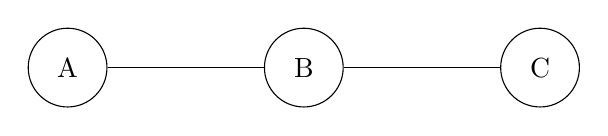
\begin{tikzpicture}
        %%%%%%%%%% Nodi %%%%%%%%%%
        \node[circle, draw, minimum size=1cm] (A) at  (0,0) {A};
        \node[circle, draw, minimum size=1cm] (B) at  (3,0) {B};
        \node[circle, draw, minimum size=1cm] (C) at  (6,0) {C};

        %%%%%%%%% Archi %%%%%%%%%%
        \draw (A) -- (B) -- (C);
    \end{tikzpicture}
\end{center}

            Situazione iniziale: $D_{AC} = 2 e D_{BC} = 1$.

            Il link $\overline{BC}$ diventa inutilizzabile, B riceve il DV di A che contiene l'informazione $D_{AC} = 2$, per cui esso computa una nuova $D_{BC} = D_{BA} + D_{AC} = 3$ e lacomunica ad A.

            A calcola la nuova distanza $D_{AC} = D_{AB} + D_{BC} = 4$.

            Il processo continua all'infinito.

            Sono stati proposti vari rimedi, ma nessuno risolutivo.

        \subsubsection{RIP Protocol}
            \textbf{RIP (Routing Information Protocol)} è la prima implementazione di un protocollo DV.
        
            Caratteristiche del protocollo RIP:
            \begin{itemize}
                \item Metrica: basata solo sulla minimizzazione degli hops (massimo 15).
                \item Nodi RIP attivi (tipicamente router): annunciano i loro percorsi, avviene ogni 30 secondi e quando si verificano aggiornamenti.
                \item Nodi RIP passivi (tipicamente host): aggiornano senza annunciare.
            \end{itemize}
        
        \subsubsection{Protocollo Link State}
            Si tratta di un \textit{routing protocol} in cui ogni nodo determina e mantiene aggiornata la topologia della rete da cui calcola la \textit{routing table}, applicando un \textit{routing algorithm}.

            Il protocollo si sviluppa nelle seguenti fasi:
            \begin{enumerate}
                \item Scoperata dei vicini (neighbor greetings): invio di un pacchetto HELLO su tutte le linee.
                \item Misurazione costo linea: invio di un pacchetto ECHO ai router che hanno risposto all'HELLO.
                \item Costruzione di un pacchetto (\textbf{Link State Packet: LSP}) con tutte le informazioni ricavate nella fase precedente: l'identità del trasmittente, il numero di sequenza, l'età e la lista dei vicini con il relativo ritardo misurato.
                \item Distribuzione periodica del LSP a tutti i nodi della rete, con un numero di sequenza, utilizzando l'algoritmo di flooding.
                
                Se arriva un pacchetto con un numero di sequenza inferiore al numero più alto visto fino a quel momento, il pacchetto viene scartato (è ritenuto obsoleto).
                \item Ogni nodo, dopo aver ricevuto gli LSP da tutti gli altri, costruisce la topologia della rete ed applica un routing algorithm (SPF) per il calcolo della tabella.
            \end{enumerate}

        \subsubsection{Esempio di Protocollo Link State}
            \begin{center}
    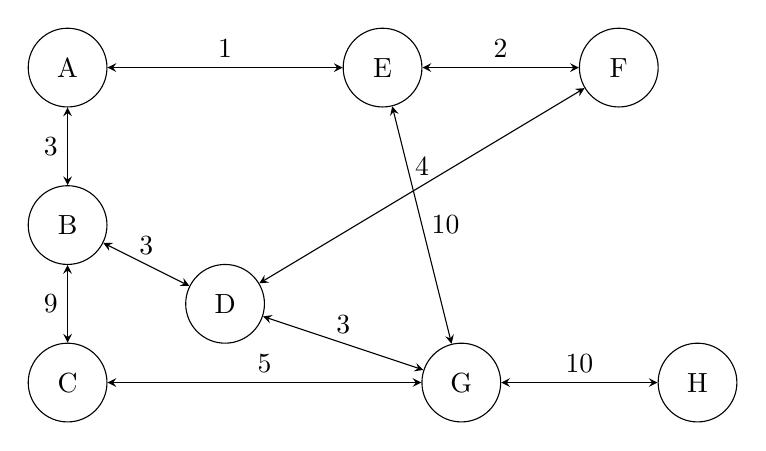
\begin{tikzpicture}
        %%%%%%%%%% Nodi %%%%%%%%%%
        \node[circle, draw, minimum size=1cm] (A) at  (0,4) {A};
        \node[circle, draw, minimum size=1cm] (B) at  (0,2) {B};
        \node[circle, draw, minimum size=1cm] (C) at  (0,0) {C};
        \node[circle, draw, minimum size=1cm] (D) at  (2,1) {D};
        \node[circle, draw, minimum size=1cm] (E) at  (4,4) {E};
        \node[circle, draw, minimum size=1cm] (F) at  (7,4) {F};
        \node[circle, draw, minimum size=1cm] (G) at  (5,0) {G};
        \node[circle, draw, minimum size=1cm] (H) at  (8,0) {H};
        
        %%%%%%%%% Archi %%%%%%%%%%
        \draw[<->,>=stealth] (A) -- node[left] {3} (B);
        \draw[<->,>=stealth] (A) -- node[above] {1} (E);
        \draw[<->,>=stealth] (B) -- node[left] {9} (C);
        \draw[<->,>=stealth] (B) -- node[above] {3} (D);
        \draw[<->,>=stealth] (C) -- node[above] {5} (G);
        \draw[<->,>=stealth] (D) -- node[above] {4} (F);
        \draw[<->,>=stealth] (D) -- node[above] {3} (G);
        \draw[<->,>=stealth] (E) -- node[above] {2} (F);
        \draw[<->,>=stealth] (E) -- node[right] {10} (G);
        \draw[<->,>=stealth] (G) -- node[above] {10} (H);
    \end{tikzpicture}
\end{center}

            Avviene una raccolta di informazioni tramite i pacchetti HELLO, ECHO. Successivamente vengono propagate le informazioni ottenute (LSP) tramite flooding.

            Per il nodo D il pacchetto sarebbe:

            \begin{table}[h]
                \centering
                \begin{tabular}{|c|c|}
                \hline
                \rowcolor[HTML]{000000} 
                {\color[HTML]{EFEFEF} \textbf{Adiacente}} & {\color[HTML]{EFEFEF} \textbf{Costo}} \\ \hline
                B & 3 \\ \hline
                F & 4 \\ \hline
                G & 3 \\ \hline
                \end{tabular}
            \end{table}

            Viene determinata la mappa della rete fornendo ogni LSP, e viene memorizzata in una LSP base dati del formato mostrato in tabella:

            \begin{table}[h]
                \centering
                \begin{tabular}{|c|c|c|c|}
                \hline
                A & B/3 & E/1 &  \\ \hline
                B & A/3 & C/9 & D/3 \\ \hline
                C & B/9 & G/5 &  \\ \hline
                D & B/3 & F/4 & G/3 \\ \hline
                E & A/1 & F/2 & G/10 \\ \hline
                F & D/4 & E/2 &  \\ \hline
                G & C/5 & D/3 & E/10 \\ \hline
                H & D/3 &  &  \\ \hline
                \end{tabular}
            \end{table}

            Il calcolo della tabella di instradamento si riduce ora al calcolo dello spanning tree di tipo SPF (Shortest Path First) e lo si effettua tramite il noto algoritmo di Dijkstra.

            Lo spanning tree ad esempio del nodo D risulterà come nella figura a lato e a seguire, la relativa tabella di instradamento.

            \begin{center}
    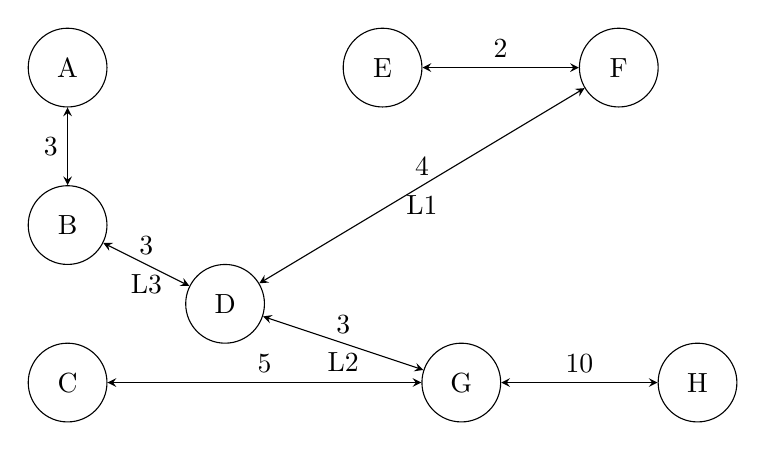
\begin{tikzpicture}
        %%%%%%%%%% Nodi %%%%%%%%%%
        \node[circle, draw, minimum size=1cm] (A) at  (0,4) {A};
        \node[circle, draw, minimum size=1cm] (B) at  (0,2) {B};
        \node[circle, draw, minimum size=1cm] (C) at  (0,0) {C};
        \node[circle, draw, minimum size=1cm] (D) at  (2,1) {D};
        \node[circle, draw, minimum size=1cm] (E) at  (4,4) {E};
        \node[circle, draw, minimum size=1cm] (F) at  (7,4) {F};
        \node[circle, draw, minimum size=1cm] (G) at  (5,0) {G};
        \node[circle, draw, minimum size=1cm] (H) at  (8,0) {H};
        
        %%%%%%%%% Archi %%%%%%%%%%
        \draw[<->,>=stealth] (A) -- node[left] {3} (B);
        \draw[<->,>=stealth] (B) -- node[above] {3} node[below] {L3} (D);
        \draw[<->,>=stealth] (C) -- node[above] {5} (G);
        \draw[<->,>=stealth] (D) -- node[above] {4} node[below] {L1} (F);
        \draw[<->,>=stealth] (D) -- node[above] {3} node[below] {L2} (G);
        \draw[<->,>=stealth] (E) -- node[above] {2} (F);
        \draw[<->,>=stealth] (G) -- node[above] {10} (H);
    \end{tikzpicture}
\end{center}

            \begin{table}[h]
                \centering
                \begin{tabular}{|c|c|}
                \hline
                A & L3 \\ \hline
                B & L3 \\ \hline
                C & L2 \\ \hline
                E & L1 \\ \hline
                F & L1 \\ \hline
                G & L2 \\ \hline
                H & L2 \\ \hline
                \end{tabular}
            \end{table}

            L'algoritmo può gestire reti di grandi dimensioni grazie alla sua rapida convergenza ed il suo comportamento è prevedibile, poiché ogni nodo ha in memoria la mappa intera della rete.

            Difficilmente si generano loop e, comunque, risulta facile identificarli ed eliminarli.

        \subsubsection{OSPF}
            Il protocollo \textbf{OSPF (Open Shortest Path First)} è di tipo Link State Packet, ed è raccomandato da IETF per Internet.

            Ogni router costruisce un pacchetto con l'elenco delle linee attive e dei loro costi (1/larghezza di banda della linea).

            Invia in flooding pacchetti \textbf{Link State Update} (multicast 244.0.0.5), questi pacchetti vengono riscontrati con un \textbf{Link State Ack}.

            Un router può chiedere informazioni con \textbf{Link State Request}.

            Se, in base ai pacchetti di update ricevuti, si sono verificate modifiche della topologia, ricalcola la tabella di routing con l'algoritmo SPF.

            Ha un rapido tempo di convergenza.

            Prevede un'organizzazione gerachica dell'AS in \textbf{aree}:
            \begin{itemize}
                \item Ogni AS-OSPF contiene almeno un'area: l’area di backbone (\verb:0.0.0.0:)
                \item Le eventuali altre aree sono connesse al Backbone.
                \item Ogni router mantiene informazioni solo riguardo alla tipologia della propria area.
            \end{itemize}
        
        \subsubsection{Protocolli Gerarchici}
            Nel caso di reti di grandi dimensioni non è possibile gestire le tabelle di routing per l'intera rete in tutti i router, in questo caso il routing deve essere gerarchico: la rete viene ripartita in aree, chiamate \textbf{Autonomous-System (AS)}.

            I router all'interno di un area sono in grado di effettuare l'instradamento relativamente alla sola area, per destinazioni al di fuori dell'area si limitano ad inviare i pacchetti a dei router "di bordo" che sono a conoscenza della topologia esterna dell'area. I router "di bordo" si occupano solamente dell'instradamento dei pacchetti fra aree.

            In linea di principio la ripartizione può essere effettuata tante volte quante si vuole, creando più livelli nella gerarchia di routing.

            \begin{center}
                \includegraphics[scale=0.45]{chapters/4/assets/schema_w.png}
            \end{center}

        \subsubsection{Protocolli di routing in Internet}
            In TCP/IP i router sono suddivisi in due classi, \textbf{Exterior Router} ed \textbf{Interior Router}.
        
            I primi interconnettono due insiemi di reti distinti. Ogni insieme di reti, gestito da una singola autorità amministrativa, è un Autonomous System ed i router interni ad essi sono proprio gli Interior.
        
            Un sistema è detto autonomo, poiché è libero di scegliere un'architettura di instradamento interna, ma deve raccogliere informazioni su tutte le sue reti e progettare uno o più gateway, gli Exterior Router, che passino le informazioni di raggiungibilità ad altri sistemi autonomi.
        
            Gli Exterior Router utilizzano protocolli denominati \textbf{EGP (Exterior Gateway Protocol)}, mentre gli Interior Router scambiano informazioni di instradamento tramite gli \textbf{IGP (Interior Gateway Protocol)}.
        
            I protocolli IGP più utilizzati sono RIP (Distance Vector) e OSPF (Link State). BGP è il protocollo raccomandato in Internet per l'interconnessione di Autonomous System.

        \subsubsection{BGP}
            \textbf{BGP (Border Gateway Protocol}, è un protocollo Path Vector: invece di propagare i costi, propaga la sequenza di AS da attraversare per arrivare alla destinazione.

            \begin{center}
                \includegraphics[scale=0.4]{chapters/4/assets/schema_x.png}
            \end{center}